\documentclass[14pt]{extreport}
\usepackage{cmap}
\usepackage[utf8]{inputenc}
\usepackage[english,ukrainian]{babel}
\usepackage{graphicx}
\usepackage{geometry}
\usepackage{listings}
\usepackage{amsmath}
\usepackage{float}
\geometry{
	a4paper,
	left=20mm,
	right=20mm,
	top=20mm,
	bottom=20mm
}
\lstset{
	columns=fullflexible, 
	frame=single, 
	breaklines=true, 
	tabsize=4,
	postbreak=\raisebox{0ex}[0ex][0ex]{\ensuremath{\hookrightarrow\space}},
	showstringspaces=false,% no symbol for spaces in strings
}
\graphicspath{ {./pictures} }
\setlength{\parindent}{4em}

\newcommand\subject{Бази даних}
\newcommand\lecturer{асистент кафедри ПЗ\\Білоіваненко М.В.}
\newcommand\teacher{асистент кафедри ПЗ\\Білоіваненко М.В.}
\newcommand\mygroup{ПЗ-32}
\newcommand\lab{8}
\newcommand\theme{Транзакції}
\newcommand\purpose{Створити простий додаток на обраній мові програмування, що виконує декілька запитів на СУБД. Відобразити в інтерфейсі результати однієї вибірки з умовами по введених параметрах. Отримати дані в інтерфейсі для одного запиту оновлення або додавання даних.}

\begin{document}
\begin{normalsize}
	\begin{titlepage}
		\thispagestyle{empty}
		\begin{center}
			\textbf{МІНІСТЕРСТВО ОСВІТИ І НАУКИ УКРАЇНИ\\
				НАЦІОНАЛЬНИЙ УНІВЕРСИТЕТ "ЛЬВІВСЬКА ПОЛІТЕХНІКА"}
		\end{center}
		\begin{flushright}
			Інститут \textbf{КНІТ}\\
			Кафедра \textbf{ПЗ}
		\end{flushright}
		\vspace{200pt}
		\begin{center}
			\textbf{ЗВІТ}\\
			\vspace{10pt}
			До лабораторної роботи № \lab\\
			\textbf{На тему}: “\textit{\theme}”\\
			\textbf{З дисципліни}: “\subject”
		\end{center}
		\vspace{40pt}
		\begin{flushright}
			
			\textbf{Лектор}:\\
			\lecturer\\
			\vspace{10pt}
			\textbf{Виконав}:\\
			
			студент групи \mygroup\\
			Коваленко Д.М.\\
			\vspace{10pt}
			\textbf{Прийняв}:\\
			
			\teacher\\
			
			\vspace{28pt}
			«\rule{1cm}{0.15mm}» \rule{1.5cm}{0.15mm} 2023 р.\\
			$\sum$ = \rule{1cm}{0.15mm}……………\\
			
		\end{flushright}
		\vspace{\fill}
		\begin{center}
			\textbf{Львів — 2023}
		\end{center}
	\end{titlepage}
		
	\begin{description}
		\item[Тема.] \theme.
		\item[Мета.] \purpose.
	\end{description}

	\section*{Лабораторне завдання}
Створити простий додаток на обраній мові програмування, що виконує декілька запитів на СУБД. Відобразити в інтерфейсі результати однієї вибірки з умовами по введених параметрах. Отримати дані в інтерфейсі для одного запиту оновлення або додавання даних.

Виконати виклик раніше створеної збереженої процедури.

На 4 бали: врахувати помилки від СУБД при виконанні запитів (наприклад, некоректний формат значень або спроба порушення цілісності). Проінформувати користувача, зробити відкат транзакції та виконати повторну спробу. Розробити два різних сценарії обробки помилок.

На 7 балів: створити умови конкуруючого виконання транзакцій при оновленні даних, які викликають конфлікт. Проаналізувати тип аномалії. Знайти рішення, щоб при збереженні умов випадок конфлікту був врегульований. Розробити сценарій обробки помилки, при якому відкат та повторне виконання транзакції є обґрунтованим.
	
	
	\section*{Хід роботи}
	\begin{figure}[H]
		\centering
		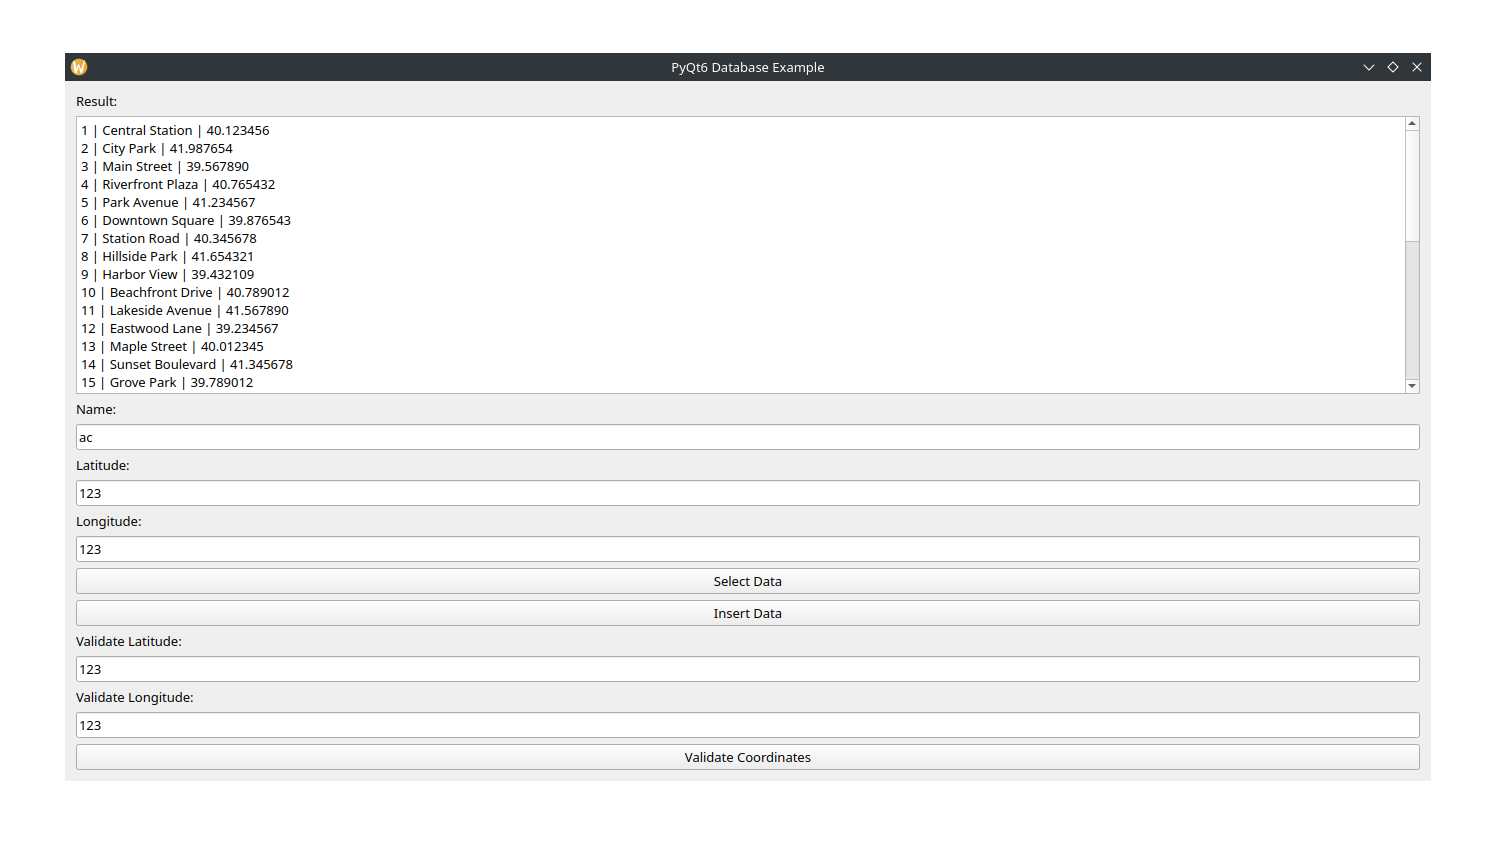
\includegraphics[scale=0.45]{1}
		\caption{Робота програми}
	\end{figure}
	
	
	\section*{Висновок}
	Під час виконання лабораторної роботи я створив простий додаток на обраній мові програмування, що виконує декілька запитів на СУБД. Відобразив в інтерфейсі результати однієї вибірки з умовами по введених параметрах. Отримав дані в інтерфейсі для одного запиту оновлення або додавання даних.
	 
\end{normalsize}
\end{document}
